\documentclass[journal]{IEEEtran}

\usepackage{cite}
\usepackage{amsmath}
\interdisplaylinepenalty=2500
\usepackage{algorithm}
\usepackage[noend]{algpseudocode}
\usepackage{array}
\usepackage{graphicx}
\usepackage{float}
\usepackage{lipsum}
\usepackage{hyperref}

% correct bad hyphenation here
\hyphenation{op-tical net-works semi-conduc-tor}


\begin{document}
\title{Analysis of camera calibration techniques for the concentric circles pattern}

\author{Wilbert~Pumacay,~\textit{Catholic University San Pablo},~wilbert.pumacay@ucsp.edu.pe\\
        Gerson~Vizcarra,~\textit{Catholic University San Pablo},~gerson.vizcarra@ucsp.edu.pe}

% make the title area
\maketitle

\begin{abstract}
This paper presents an algorithm for camera calibration using the concentric circles pattern, using a robust pipeline for detection, and further refinement based on the refinement process presented by Prakash \cite{Prakash2012}. We present a comparison with OpenCV's pattern detection functionality, which consists of the chessboard and circle grid pattern detectors; and analyze the results using the refinement process mentioned earlier, to check if there are any improvements by using the refinement process.
\\
\\
We also analyze how the selection of the frames and poses for the camera calibration process can lead to undesired results if done incorrectly by showing how poor distributions lead to bad calibration results.
\end{abstract}

\begin{IEEEkeywords}
Camera calibration, calibration pattern, concentric circles, image processing.
\end{IEEEkeywords}


\section{Introduction}

\IEEEPARstart{T}{he} camera calibration process is an important step in several applications, like augmented reality. To do calibration properly using current calibration methods we need to get features we can related in both 2D camera space and 3D world space to estimate the camera parameters that give this mapping. In this context, the use of grid patterns help by giving us the features we need, being the components in the pattern which we must detect in every frame in video.
\\
\\
The camera calibration problem consists of finding 11 parameters that describe the mapping between 2D camera space and 3D world space. Six parameters, called extrinsic, come from an homogeneous transform, giving 6 parameters ( rotation and translation around the axes ). The other 5 parameters, called intrinsic, define some internal properties of the camera. This can be expressed in the following transformation equation:

\begin{equation}
  \begin{bmatrix}
    \mu \\
    \nu \\
      1
  \end{bmatrix} =
  \begin{bmatrix}
    \alpha & \gamma & \mu_{0} \\
       0   & \beta  & \nu_{0} \\
       0   &    0   &    1
  \end{bmatrix}
  \begin{bmatrix}
    r_{x_{1}} & r_{y_{1}} & r_{z_{1}} & t_{x}\\
    r_{x_{2}} & r_{y_{2}} & r_{z_{2}} & t_{y}\\
    r_{x_{3}} & r_{y_{3}} & r_{z_{3}} & t_{z}
  \end{bmatrix}
  \begin{bmatrix}
    x \\
    y \\
    z \\
    1
  \end{bmatrix}
%
\end{equation}

In this equation we can detail each of the variables: $x,y,z$ are original coordinates of an object, $r_{ij}$ and $t_{ij}$ means the rotation and translation values respectively in the model matrix, $\alpha$ and $\beta$ represents the focal length in x and y axis respectively, $\mu_0$ and $\nu_0$ are the coordinates x and y at the optical center.
\\
\\
To find these parameters, camera calibration methods make use of correspondences between 2D and 3D spaces in order to fit the parameters that best describe this mapping. We achieve this by minimizing the following function:

\begin{equation}
  \sum^{m}_{i} \sum^{n}_{j} \Vert TP^{ij}_{3D} - P^{ij}_{2D} \Vert^{2}
\end{equation}

Where we are trying to minimize the difference between the expected projection and the actual projection over some set of features. The key idea is that supplying sufficient features that have a correct mapping, we can get the 11 parameters needed that minimize this function. So, a key part is the detection of these features.
\\
\\
In equation $2$ we are looping through a set of features $n$ that are found in each frame of a video of $m$ frames, so, we basically need to detect some feature points in each frame of video, which is achieved by a pattern detector. We implemented a detector for the concentric rings pattern for this purpose.
\\
\\
Once calibrated, we can try to further improve the results of the calibration process by using the previous calibration data, which is used to correct the distortion and calculate a new refined set of features by running the pattern detector in a region which is parallel to the camera plane ( fronto parallel transformation ).

\section{About the method}
The general structure of the implemented pipeline is shown in Fig. 1. There are two main steps in the pipeline, which are depicted with a different color each.
\\
\\
\begin{itemize}
  \item \textbf{Initial calibration process}, which is in charge of detecting the pattern in the original frames from video. In this step we use our pattern detector, which handles the extraction of the pattern from the original images. We also create a batch from this detected patterns, by using a manual picking method for selecting the batch for the initial calibration.
  \item \textbf{Refinement process}, in which we use the initial batch from the initial calibration process, and perform a fronto-parallel transformation, by finding a homography matrix between the pattern corners and a fronto-parallel view of the pattern. Once in this fronto-parallel view, we can take advantage of a simpler, which allows us to detect the pattern more accurately.
\end{itemize}

\begin{figure}[H]
\centering
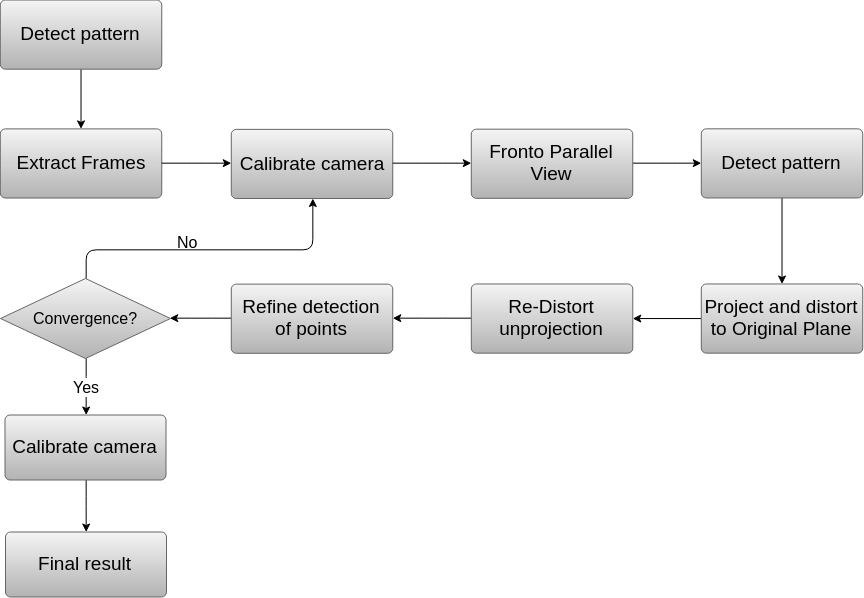
\includegraphics[width=3.0in]{_img/img_report4_pipeline.png}
\caption{Pipeline of the implementation.}
\end{figure}

\subsection{ \textbf{ Initial calibration } }

We first discuss the initial calibration process, which consists of out pattern detector and the calibration batch picking process.

\subsubsection{ \textbf{Circle concentric pattern detection} }
In order to detect the pattern faster and get better results, we created a state based detector, with three main modes ( See Fig. 2 ):
\\
\begin{itemize}
  \item \textbf{Finding Mode}, which is in charge of detecting the pattern using an initial region of interest.
  \item \textbf{Tracking Mode}, which tracks the pattern by following each frame based on the previous.
  \item \textbf{Recovering Mode}, which is a temporal mode in charge of detecting the pattern from scratch in case tracking was lost.
\end{itemize}

\begin{figure}[H]
\centering
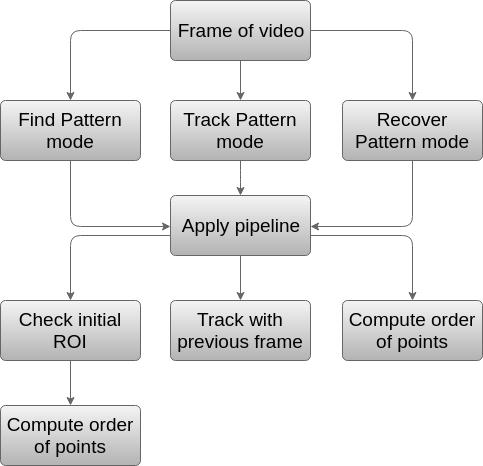
\includegraphics[width=2.3in]{_img/img_report4_pipeline_modes.png}
\caption{Behavior of mode based detector.}
\end{figure}

For detecting the points in pattern we used a detection pipeline using some OpenCV functionality. This pipeline is shown in Fig. 3.

\begin{figure}[H]
\centering
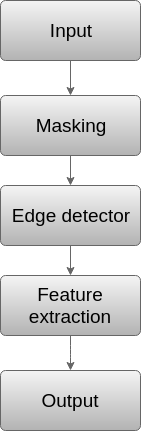
\includegraphics[width=0.7in]{_img/img_report4_pipeline_detector.png}
\caption{Detection pipeline}
\end{figure}

We now will show in more detail what each step in this pipeline does.
\\
\begin{itemize}
    \item \textbf{Trehsholding}
        \\
        \\
        This step is in charge of isolating the pattern by using thresholding operations. The approach consists on creating a mask from the grayscale transformed image applying \textbf{Adaptive Thresholding algorithm}, this algorithm relies on Integral Image technique specified in \cite{IntegralImageThresholding}.
        \begin{algorithm}
        \caption{Trehsholding}
        \label{alg:mask2}
        \begin{algorithmic}[1]
        \State $\textit{Set up thresholding parameters}$
        \State $mask   = \textit{rgb2gray}( inputImage )$
        \State $mask   = \textit{AdaptiveThreshold}(mask, blockSize)$\\
        \Return $masked$
        \end{algorithmic}
        \end{algorithm}
        %%%%%%%%%%%%%%%%%%%%%%%%%%%%%%%%%%%%%%%%%%%%%%%%%%%%%%%
        \begin{figure}[H]
        \centering
        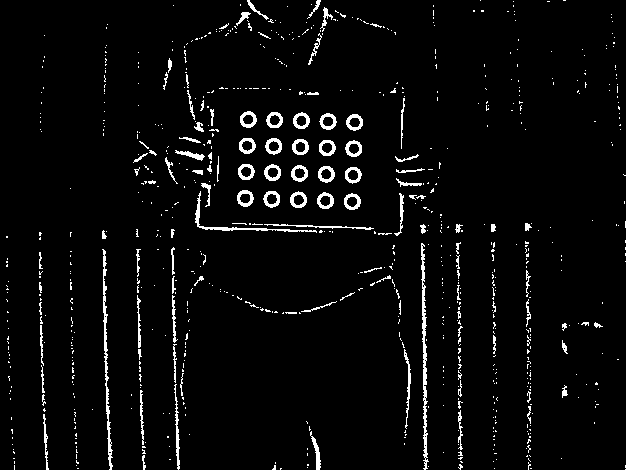
\includegraphics[width=2.5in]{_img/report_4/img_pipeline_detection_mask.png}
        \caption{Thresholding step}
        \end{figure}

    \item \textbf{Edge detection}
        \\
        \\
        In this stage of the pipeline we extract edges from the result of the previous stage. In order to do this, we applied \textbf{Scharr operators} on \textit{x} and \textit{y} axis (as described in algorithm 2); Scharr is the result from Sobel algorithm minimizing weighted mean squared angular error in Fourier domain.
        %% TODO: Gerson
        \begin{algorithm}
        \caption{Edge detection}
        \begin{algorithmic}[1]
        \State $axis_x   = \textit{Scharr}(masked, 1, 0)$
        \State $axis_x   = \textit{Abs}(axis_x)$
        \State $axis_y   = \textit{Scharr}(masked, 0, 1)$
        \State $axis_y   = \textit{Abs}(axis_y)$
        \State $edgesImage   = \textit{Add}(axis_x, axis_y)$ \\
        \Return $edgesImage$
        \end{algorithmic}
        \end{algorithm}

        \begin{figure}[H]
        \centering
        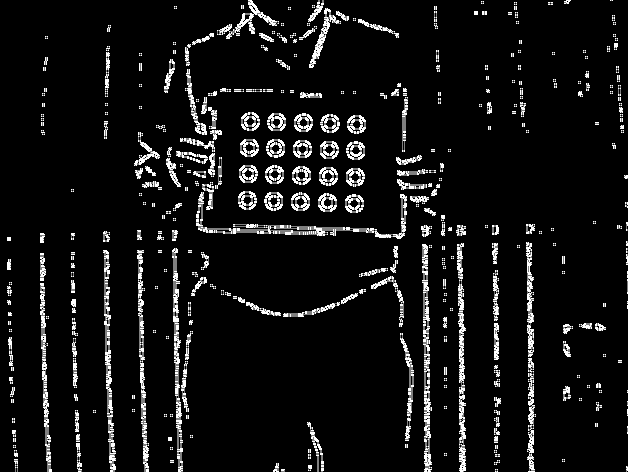
\includegraphics[width=2.5in]{_img/report_4/img_pipeline_detection_edges.png}
        \caption{Edge detection to mask.}
        \end{figure}

    \item \textbf{Feature extraction}
        \\
        \\
        The last stage consist of extracting the features needed for the calibration from the edges detected in the previous stage. We used OpenCV's \textbf{SimpleBlobDetector} that applies an extra thresholding on the image, applies the \textbf{findContours} algorithm to calculate the blob centers, groups centers of several images by their coordinates in blobs and finally, estimates the final centers of the blobs. For detecting only pattern blobs, we had to apply similar heuristics to above (color blobs, area, aspect ratio, and convexity of points).

        \begin{figure}[H]
        \centering
        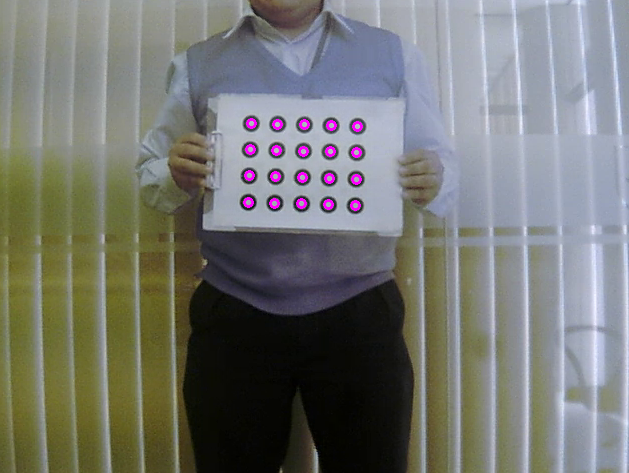
\includegraphics[width=2.5in]{_img/report_4/img_pipeline_detection_blobs.png}
        \caption{Result after feature detection.}
        \end{figure}
\end{itemize}

\subsubsection{ \textbf{ Pattern Matching and Ordering } }
Once we have the features extracted, we have to order them for them to be used in the calibration algorithm.
\\
\\
To achieve this, we made a simple algorithm that matches the best candidate grid to the current features, and correct by the orientation in order to choose a correct ordering. We first create a bounding box of the current possible corners. Then, we take the outer most corners as the corners of the pattern.
\\
\\
With this information, we can compute a candidate grid that represents the positions where the candidate points should be, as seen in figure 7. We check for each combination of outer most corners, which ordering gives the best fit. This will give us a correct ordering of the outer most corners of the pattern.
\\
\\
\begin{figure}[H]
\centering
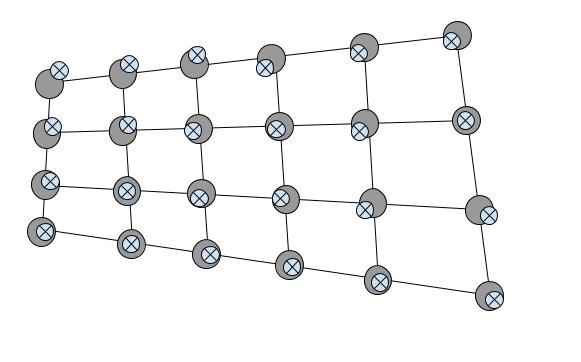
\includegraphics[width=2.5in]{_img/img_report3_pattern_matching.jpg}
\caption{Grid pattern matching.}
\end{figure}
Lastly, we check that the orientation of the board is in some range, as shown in figure 8, which will complete the corner ordering, as shown in figure 9.
\\
\\
\begin{figure}[H]
\centering
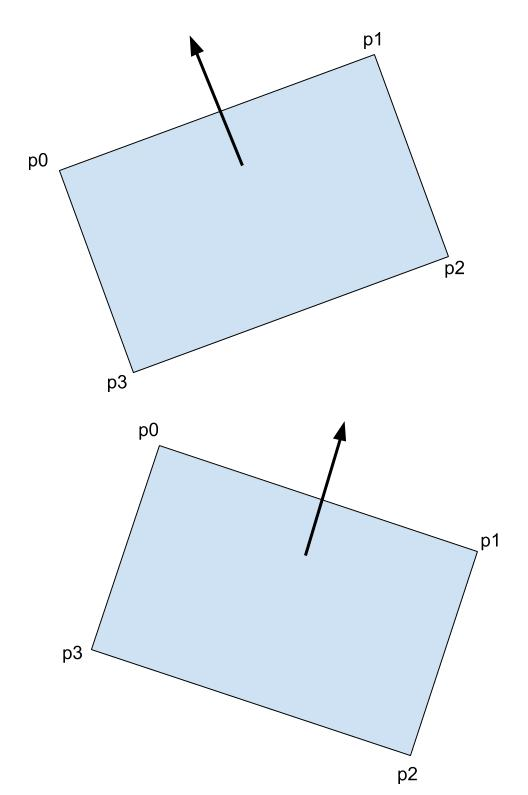
\includegraphics[width=2.5in]{_img/img_pattern_orientation_checking.jpg}
\caption{Pattern orientation check.}
\end{figure}

\begin{figure}[H]
\centering
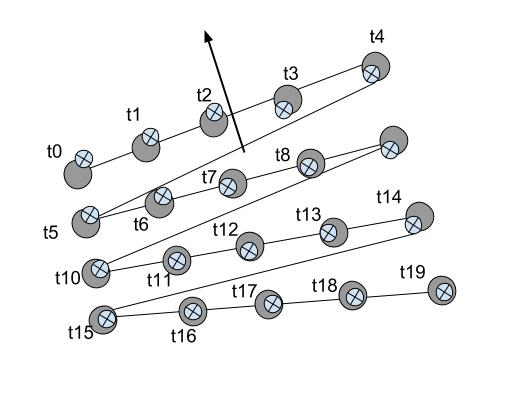
\includegraphics[width=2.5in]{_img/img_report3_pattern_order_check.jpg}
\caption{Pattern final ordering after matching.}
\end{figure}

\subsubsection{Calibration process}
For the camera calibration process, we took a batch frames were that pattern was successfully detected. We picked them manually, by using some tools we implemented in order to pick a correct distribution of frames. We implemented a heatmap like visualizer and a points distribution visualizer to check the right 2D distribution over all the field of view; and a histogram visualizer, which gave us the most picked angle at which the pattern was taken.
\\
\\
In Fig. 10 we show the heatmap and point distribution tools in a sample initial calibration process, and in Fig. 11 we show the histogram tool.

\begin{figure}[H]
\centering
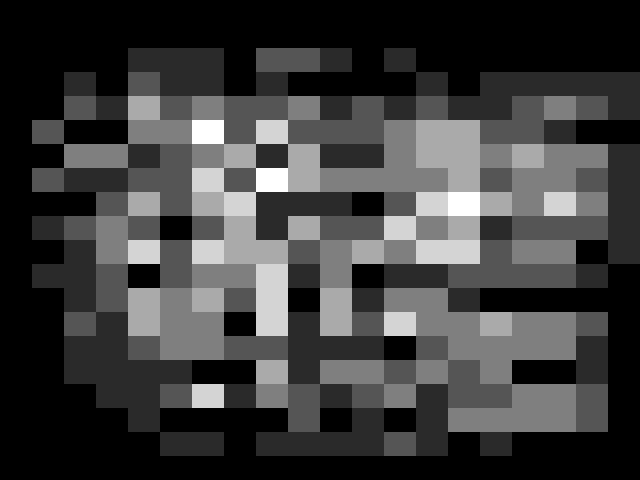
\includegraphics[width=1.5in]{_img/img_report3_heatmap.png}
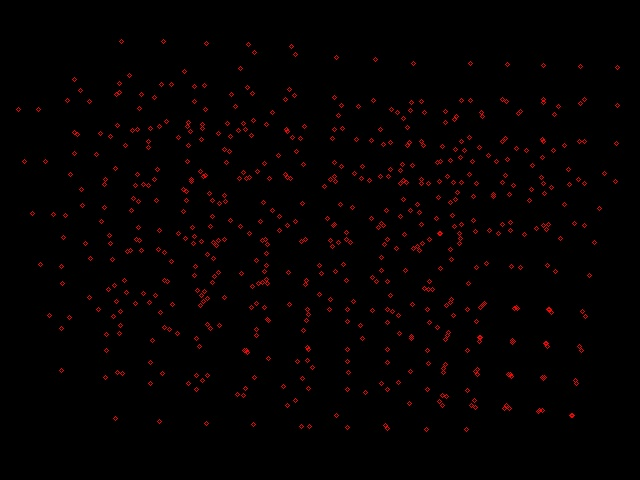
\includegraphics[width=1.5in]{_img/img_report3_points_distribution.png}
\caption{Left: Heatmap. Right: Points distribution.}
\end{figure}

\begin{figure}[H]
\centering
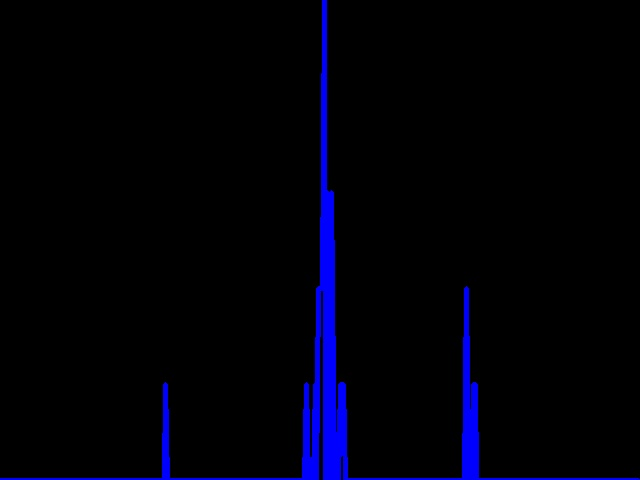
\includegraphics[width=1.5in]{_img/img_report3_angle_histogram.png}
\caption{Angle distribution histogram screen.}
\end{figure}

\subsection{ \textbf{ Refinement process } }

The second step in the calibration is the refining step, in which we use the previous calibrated batch and refine the detected points in a fronto-parallel view by means of finding an homography between the pattern in the image, and a fronto view.

\subsubsection{ \textbf{ Fronto parallel transformation } }

The pipeline for the fronto parallel transformation is depicted in Fig. 12, and consists of the following steps :

\begin{itemize}

    \item \textbf{Undistortion}
        \\
        \\
        Camera distortion can make the detector find points in the pattern that are a little off from their actual position. For example, in the case of the chessboard pattern, we could have distortion affecting the pattern in a radial way, as shown in Fig. 13.

        \begin{figure}[H]
        \centering
        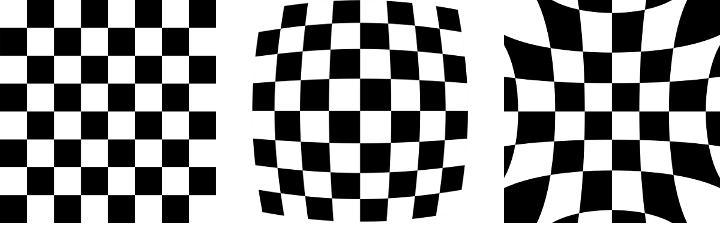
\includegraphics[width=2.5in]{_img/img_cv_distortion_examples.png}
        \caption{ \textit{ Left: Undistorted pattern. Middle: Barrel distortion. Right: Pincushion distortion. } }
        \end{figure}

        To correct for this, we use the estimated distortion coefficients from the initial camera calibration process by using OpenCV's \textbf{undistort} function, which will give us the following result.

        %% TODO: Add screenshots from the undistortion process ( distorted - undistorted pair )
        \begin{figure}[H]
        \centering
        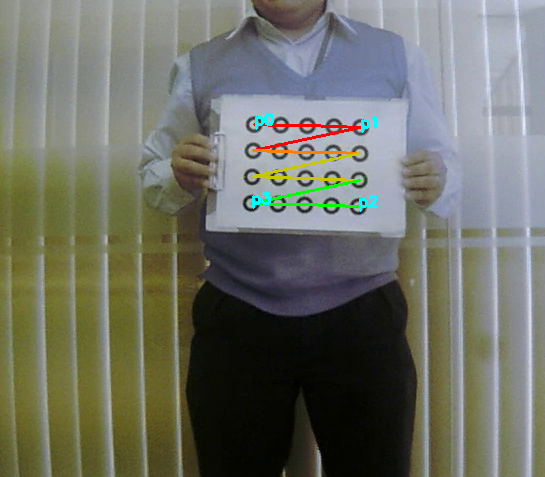
\includegraphics[width=1.5in]{_img/report_4/img_refinement_undistortion_original.png}
        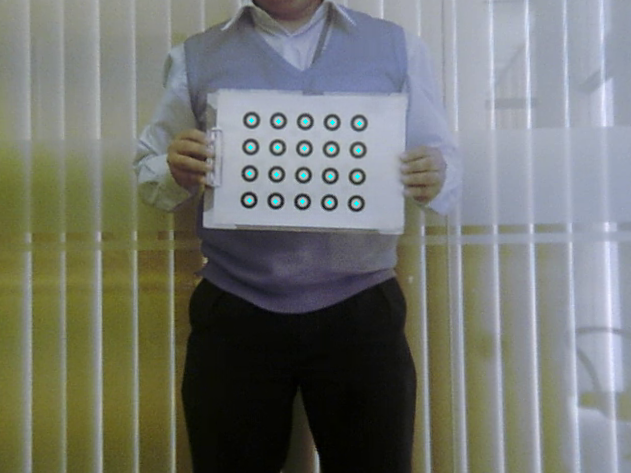
\includegraphics[width=1.5in]{_img/report_4/img_refinement_undistortion_b.png}
        \caption{Left: Original. Right: Undistorted.}
        \end{figure}

        We make sure to undistort the pattern points as well, as we need them for the fronto parallel transformation. We achieve this with OpenCV's \textbf{undistortPoints} function.
        \\
    \item \textbf{Direct fronto-parallel transformation}
        \\
        \\
        Once we are in the undistorted space, we can find the homography which will help us transform the image into a fronto-paralle view, as shown in Fig. 15.

        \begin{figure}[H]
        \centering
        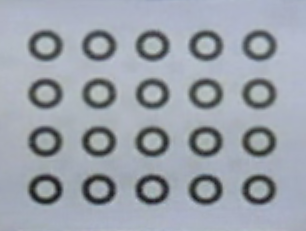
\includegraphics[width=2.5in]{_img/report_4/img_refinement_fronto_view.png}
        \caption{ \textit{ Fronto parallel view } }
        \end{figure}

        To achieve this we construct a correspondance between the corners points in the pattern ( plus some offset, to make sure the whole pattern is mapped ) and a fronto-parallel view of the pattern ( where only the whole pattern fronto-parallel to the view ). With this correspondance we find the homography transformation, by means of OpenCV's \textbf{getPerspectiveTransform} function.

        \begin{figure}[H]
        \centering
        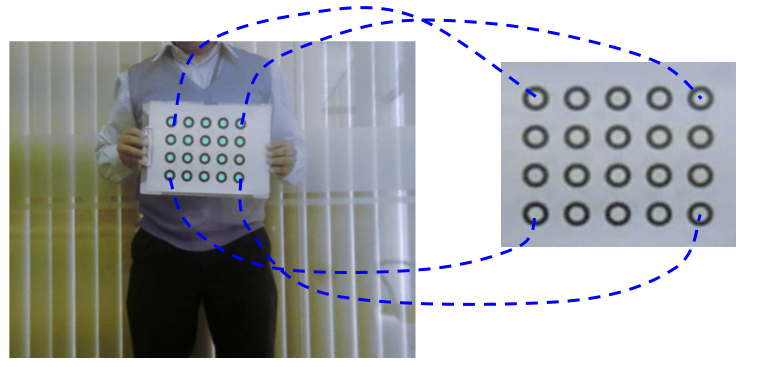
\includegraphics[width=2.5in]{_img/report_4/img_homography.png}
        \caption{Correspondance for homography computation}
        \end{figure}

        We then transform the image to a fronto parallel view by means of OpenCV's \textbf{warpPerspective} method.
        \\

    \item \textbf{Detection in the fronto-parallel space}
        \\
        \\
        Once in the fronto-parallel view, we can use the pattern detectors from the initial stage to compute a fronto-refined pattern of points. In the case of the patterns supported by OpenCV, namely the chessboard and circle grid patterns, we used the same detectors as in the initial step : \textbf{findChessboardCorners} and \textbf{findCircleGrid} detectors.
        \\
        \\
        For the concentric-rings pattern we use a different detector than our original detector. As described in Prakash's paper \cite{Prakash2012}, we use the following four-step detector :

        \begin{itemize}

            \item Adaptive thresholding
            \item Canny edges detection
            \item Contour finding and ellipse fitting
            \item Ellipse discards by heuristics and patter fitting

        \end{itemize}

        In Figs. 16 to 18, we show the results of this detection in the fronto-paralle space.

        \begin{figure}[H]
        \centering
        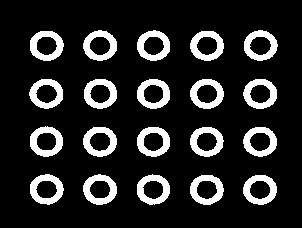
\includegraphics[width=1.0in]{_img/report_4/img_refinement_fronto_detection_mask.png}
        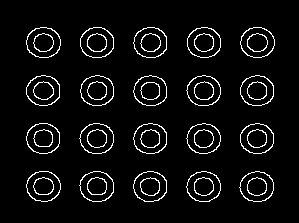
\includegraphics[width=1.0in]{_img/report_4/img_refinement_fronto_detection_edges.png}
        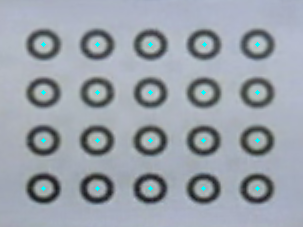
\includegraphics[width=1.0in]{_img/report_4/img_refinement_detection_features.png}
        \caption{Three steps of the detection in the fronto parallel view}
        \end{figure}

        Once we have this detected pattern, we just have to take it back to the original image space.
        \\

    \item \textbf{Inverse fronto-parallel transformation}
        \\
        \\
        We can now use the inverse of the previously found homography matrix, to take the detected points back to the undistorted space. We just use OpenCV's \textbf{perspectiveTransform} method in these points and get the pattern points in the undistorted space, as shown in Fig. 19.

        \begin{figure}[H]
        \centering
        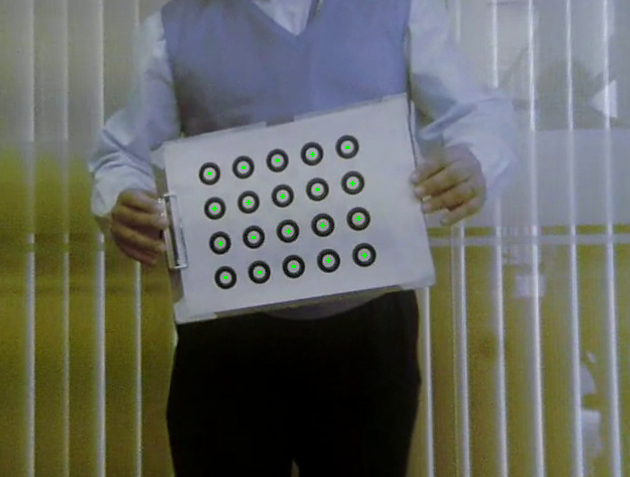
\includegraphics[width=2.5in]{_img/report_4/img_refinement_inverse_perspective.png}
        \caption{Undistorted image with refined points}
        \end{figure}

        We now just have to take these points back from the undistorted space to the original distorted image space.
        \\

    \item \textbf{Distortion}
        \\
        \\
        Here we have to implement the distortion equations using the Radial-tangential distortion model, as OpenCV doesn't provide us with a handy helper function for this task. Recall, the distortion model can be described by the following set of equations.
        \begin{gather*}
            x = ( x_{undistorted} - c_{x} ) / f_{x}\\
            y = ( y_{undistorted} - c_{y} ) / f_{y}\\
            r = \sqrt{ x^{2} + y^{2} } \\
            x_{distorted} = x ( 1 + k_{1} r^{2} + k_{2} r^{4} + k_{3} r^{6} )\\
            y_{distorted} = y ( 1 + k_{1} r^{2} + k_{2} r^{4} + k_{3} r^{6} )\\
            x_{distorted} = x_{distorted} + ( 2 p_{1} x y + p_{2} ( r^{2} + 2 x^{2} ) )\\
            y_{distorted} = y_{distorted} + ( 2 p_{2} x y + p_{2} ( r^{2} + 2 y^{2} ) )\\
            x_{new} = x_{distorted} f_{x} + c_{x}\\
            y_{new} = x_{distorted} f_{y} + c_{y}\\
        \end{gather*}

        After we applied these equations, we get the following pattern in the original view.

        \begin{figure}[H]
        \centering
        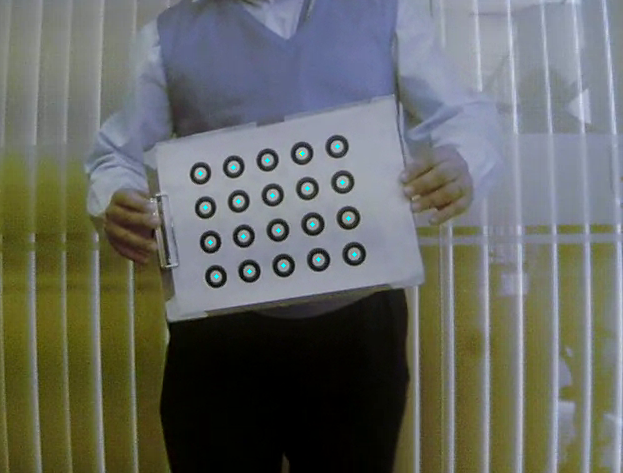
\includegraphics[width=1.5in]{_img/report_4/img_refinement_distortion.png}
        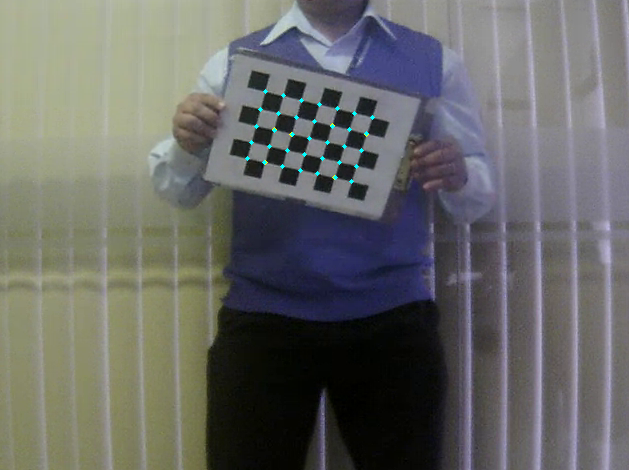
\includegraphics[width=1.5in]{_img/report_4/img_refinement_distortion_chessboard.png}
        \caption{Refined points in original uncorrected space for rings and chessboard pattern}
        \end{figure}

        This concludes the refining process, which will give us a new refined batch to calibrate with. This is done in the last part of this step.

\end{itemize}

\subsubsection{ \textbf{ Refined recalibration } }

Once we get our new refined batch, we can then recalibrate the camera and get refined intrinsic parameters. To do this we just call OpenCV's \textbf{calibrateCamera} again, with our new refined batch. We repeat this for twenty iterations and check for the reprojection error to check if there is any convergence, as you can see in the following figure.

\begin{figure}[H]
\centering
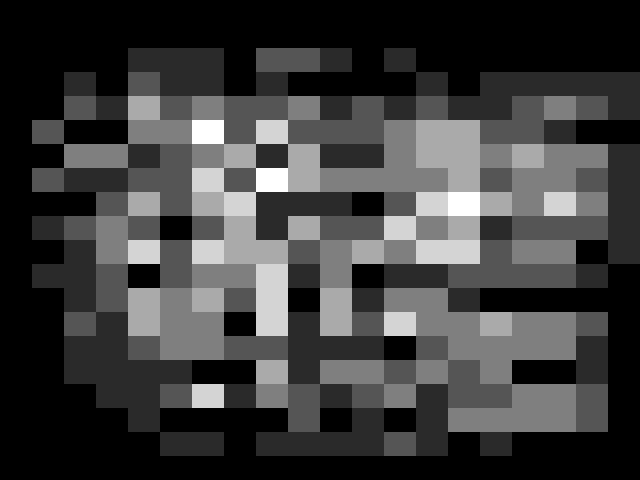
\includegraphics[width=2.5in]{_img/img_report3_heatmap.png}
\caption{Reprojection and colinearity errors during iterative recalibration}
\end{figure}

\section{Parallelization}

We got stuck in some points in the iterative process as we couldn't see intermediate results as the iterations went by. The way we tackle this issue was by making the calibration and refining processes run in separate threads, separate of the application main thread, which main purpose was data visualization.
\\
\\
This approach allowed us to analyze the results more quickly, as well as taking them quickly. A simple change can be made to make batches of refinements and calibrations run in different threads.
\\
\\
To see more of this implementation, refer to the repository and the implementation of the \href{https://github.com/wpumacay/calibcv/blob/dev/calibration/calibrationBaseDetector.cpp}(\textbf{BaseDetector}) and \href{https://github.com/wpumacay/calibcv/blob/dev/calibration/calibrationTool.h}(\textbf{Calibrator}) classes, which implement this functionality.

\section{Results}
We calibrated two cameras using as feature detection the three detection algorithms described earlier ( OpenCV's chessboard and circle finder and our algorithm )

For each calibration, we took a fixed batch of 20, 30, 40, 50 correctly processed images. The results are the following:

\begin{table}[h]
\centering
\caption{Chessboard pattern results with Lifecam camera}
\begin{tabular}{ |c||c|c|c|c|  }
 \hline
 N° Batch & \multicolumn{2}{c|}{RMS} & \multicolumn{2}{c|}{Colinearity}\\
 \cline{2-5}
 & Initial & Iterative & Initial & Iterative \\
 \hline
 20        & 0.374204 & 0.38766 & 6.46812 & 6.46958 \\
 30        & 0.415195 & 0.428411 & 7.00946 & 7.00455 \\
 40        & 0.336462 & 0.287172 & 4.33423 & 4.33893 \\
 50        & 0.306374 & 0.326697 & 5.42552 & 5.37304 \\
 \hline
\end{tabular}
\\
\end{table}

\begin{figure}[H]
\centering
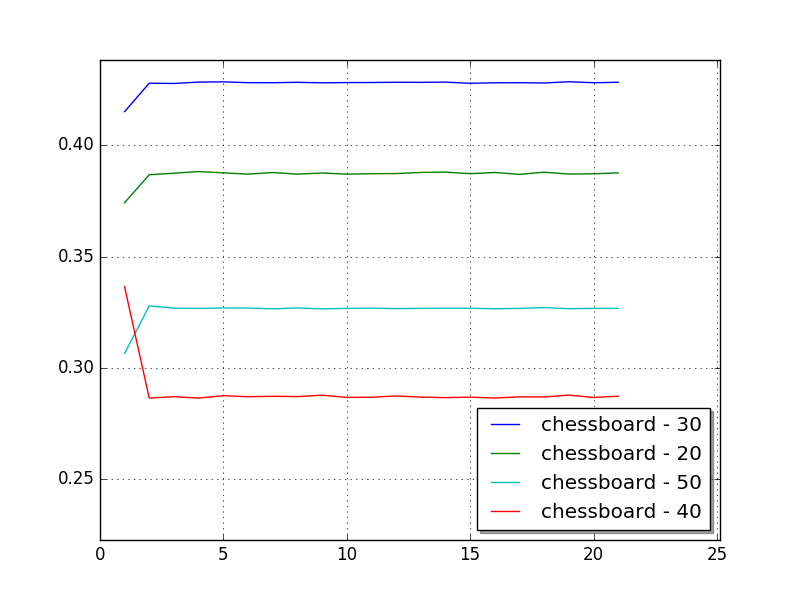
\includegraphics[width=2.5in]{_img/report_4/img_results_lifecam_chessboard.png}
\caption{Results of RMS vs iterations in Lifecam camera and chessboard pattern}
\end{figure}

\begin{figure}[H]
\centering
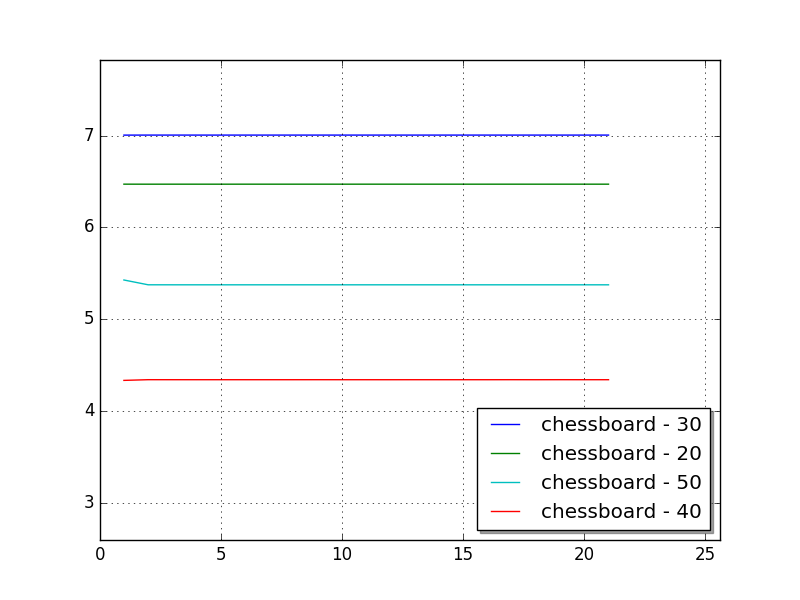
\includegraphics[width=2.5in]{_img/report_4/img_results_lifecam_colinearity_chessboard.png}
\caption{Results of colinearity error vs iterations in Lifecam camera and chessboard pattern}
\end{figure}


\begin{table}[h]
\centering
\caption{Asymmetric circles pattern results with Lifecam camera}
\begin{tabular}{ |c||c|c|c|c|  }
 \hline
 N° Batch & \multicolumn{2}{c|}{RMS} & \multicolumn{2}{c|}{Colinearity}\\
 \cline{2-5}
 & Initial & Iterative & Initial & Iterative \\
 \hline
 20        & 0.222345 & 0.222763 & 4.09431 & 4.09381 \\
 30        & 0.331330 & 0.328184 & 5.27557 & 5.3586 \\
 40        & 0.259684 & 0.248669 & 4.66493 & 4.66603 \\
 50        & 0.264687 & 0.26316 & 4.34921 & 4.28743 \\
 \hline
\end{tabular}
\\
\end{table}

\begin{figure}[H]
\centering
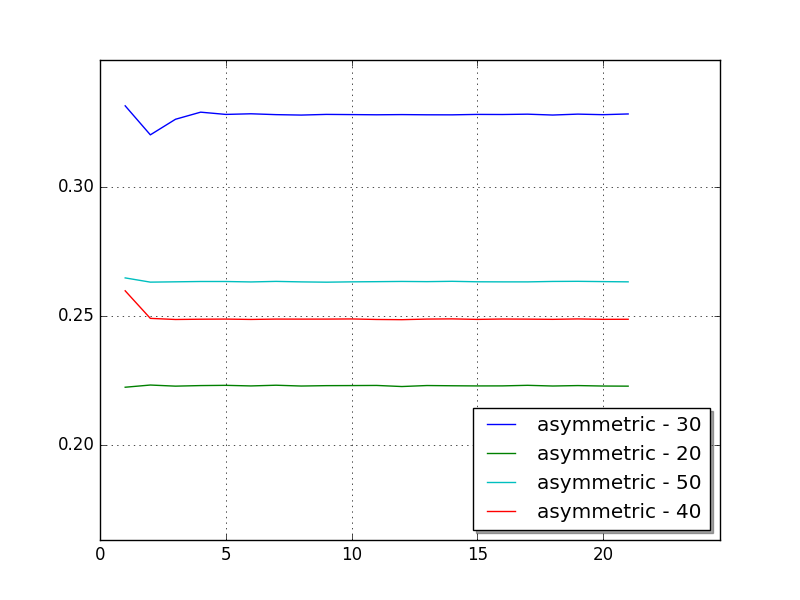
\includegraphics[width=2.5in]{_img/report_4/img_results_lifecam_asymmetric.png}
\caption{Results of RMS vs iterations in Lifecam camera and asymmetric circles pattern}
\end{figure}

\begin{figure}[H]
\centering
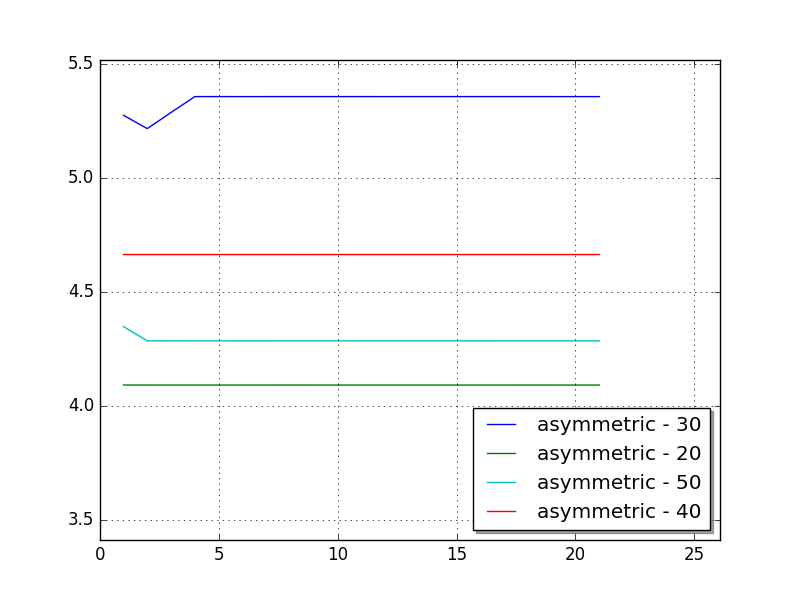
\includegraphics[width=2.5in]{_img/report_4/img_results_lifecam_colinearity_asymmetric.png}
\caption{Results of colinearity vs iterations in Lifecam camera and asymmetric circles pattern}
\end{figure}

\begin{table}[h]
\centering
\caption{Concentric circles (rings) pattern results with Lifecam camera}
\begin{tabular}{ |c||c|c|c|c|  }
 \hline
 N° Batch & \multicolumn{2}{c|}{RMS} & \multicolumn{2}{c|}{Colinearity}\\
 \cline{2-5}
 & Initial & Iterative & Initial & Iterative \\
 \hline
 20        & 0.306374 & 0.21358 & 5.42552 & 7.36297 \\
 30        & 0.259630 & 0.24536 & 7.15769 & 7.31293 \\
 40        & 0.270549 & 0.258839 & 7.63387 & 7.81084 \\
 50        & 0.374728 & 0.373889 & 8.00490 & 8.21095 \\
 \hline
\end{tabular}
\\
\end{table}

\begin{figure}[H]
\centering
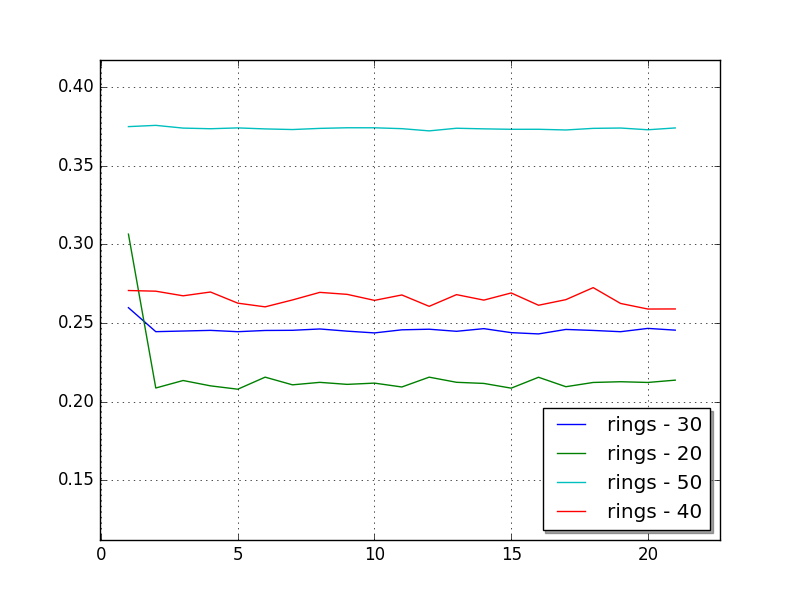
\includegraphics[width=2.5in]{_img/report_4/img_results_lifecam_rings.png}
\caption{Results of RMS vs iterations in Lifecam camera and rings pattern}
\end{figure}

\begin{figure}[H]
\centering
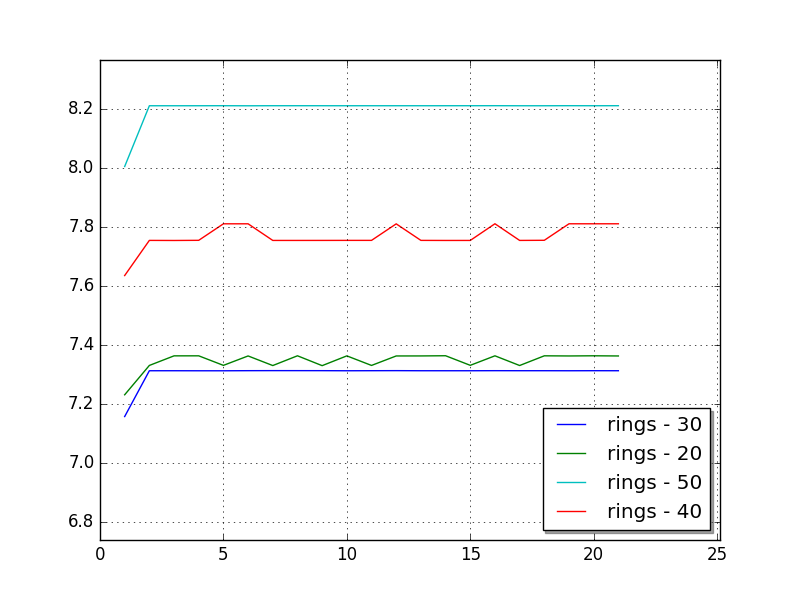
\includegraphics[width=2.5in]{_img/report_4/img_results_lifecam_colinearity_rings.png}
\caption{Results of colinearity error vs iterations in Lifecam camera and rings pattern}
\end{figure}

\begin{table}[h]
\centering
\caption{Chessboard pattern results with PS3 camera}
\begin{tabular}{ |c||c|c|c|c|  }
 \hline
 N° Batch & \multicolumn{2}{c|}{RMS} & \multicolumn{2}{c|}{Colinearity}\\
 \cline{2-5}
 & Initial & Iterative & Initial & Iterative \\
 \hline
 20        & 0.2155 & 0.2866 & 4.2983 & 4.2995 \\
 30        & 0.2272 & 0.2778 & 4.4263 & 4.4278 \\
 40        & 0.2064 & 0.2661 & 4.1667 & 4.1762 \\
 50        & 0.2487 & 0.2784 & 4.9589 & 4.9507 \\
 \hline
\end{tabular}
\\
\end{table}

\begin{figure}[H]
\centering
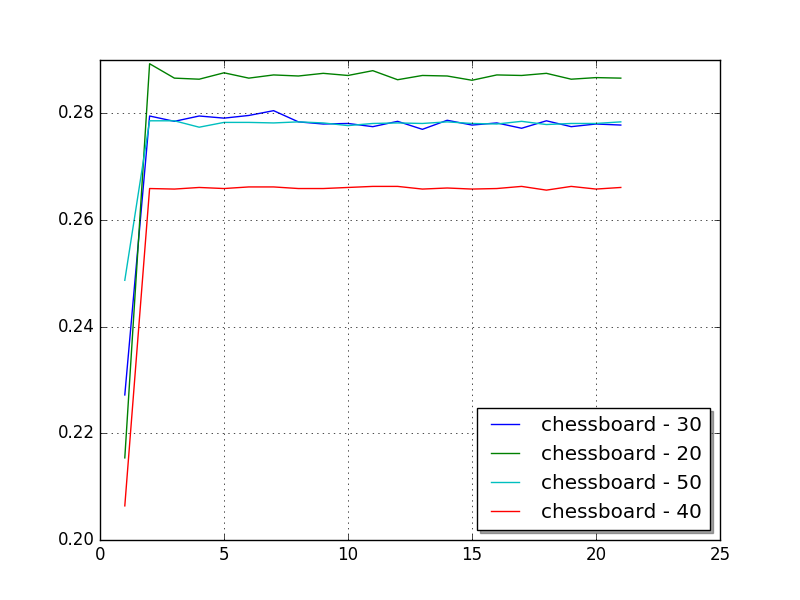
\includegraphics[width=2.5in]{_img/report_4/img_results_ps3_chessboard.png}
\caption{Results of RMS vs iterations in PS3 camera and chessboard pattern}
\end{figure}

\begin{figure}[H]
\centering
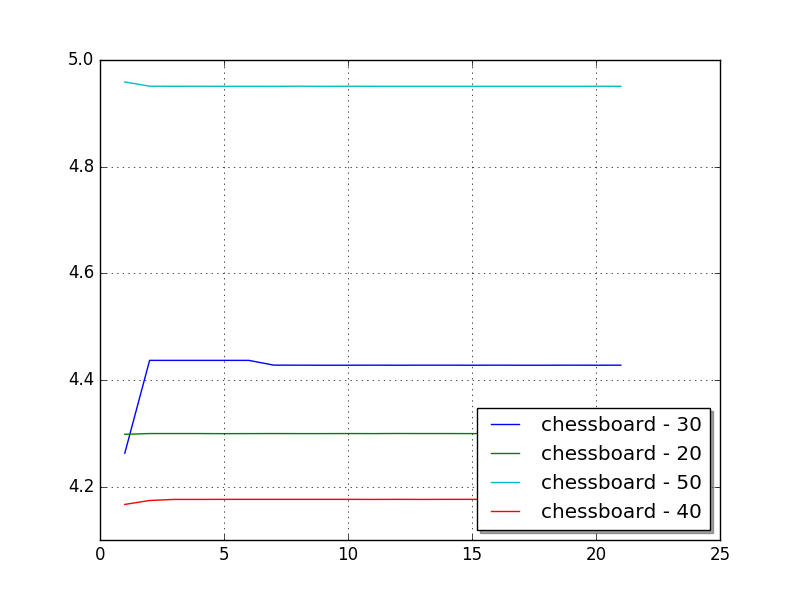
\includegraphics[width=2.5in]{_img/report_4/img_results_ps3_colinearity_chessboard.png}
\caption{Results of colinearity error vs iterations in PS3 camera and chessboard pattern}
\end{figure}

\begin{table}[h]
\centering
\caption{Asymmetric circles pattern results with Lifecam camera}
\begin{tabular}{ |c||c|c|c|c|  }
 \hline
 N° Batch & \multicolumn{2}{c|}{RMS} & \multicolumn{2}{c|}{Colinearity}\\
 \cline{2-5}
 & Initial & Iterative & Initial & Iterative \\
 \hline
 20        & 0.1914 & 0.1933 & 3.7034 & 3.7067 \\
 30        & 0.1849 & 0.1864 & 3.6823 & 3.6820 \\
 40        & 0.2625 & 0.2588 & 4.3692 & 4.3106 \\
 50        & 0.2685 & 0.2699 & 4.4143 & 4.4143 \\
 \hline
\end{tabular}
\\
\end{table}

\begin{figure}[H]
\centering
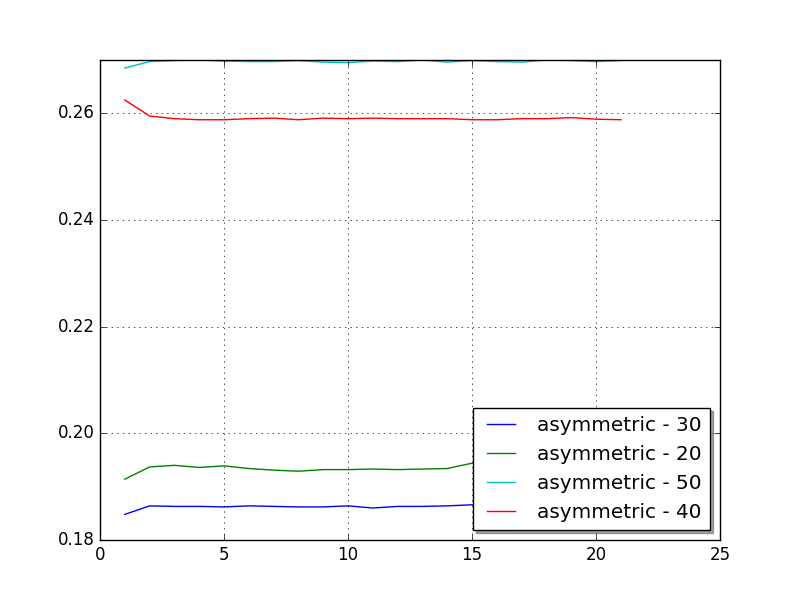
\includegraphics[width=2.5in]{_img/report_4/img_results_ps3_asymmetric.png}
\caption{Results of RMS vs iterations in PS3 camera and asymmetric circles pattern}
\end{figure}

\begin{figure}[H]
\centering
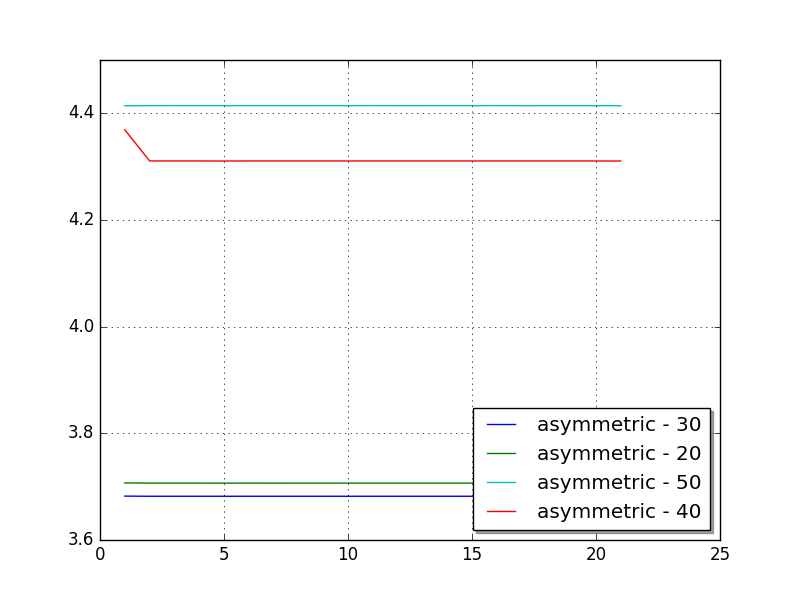
\includegraphics[width=2.5in]{_img/report_4/img_results_ps3_colinearity_asymmetric.png}
\caption{Results of colinearity error vs iterations in PS3 camera and asymmetric circles pattern}
\end{figure}

\begin{table}[h]
\centering
\caption{Concentric circles (rings) pattern results with Lifecam camera}
\begin{tabular}{ |c||c|c|c|c|  }
 \hline
 N° Batch & \multicolumn{2}{c|}{RMS} & \multicolumn{2}{c|}{Colinearity}\\
 \cline{2-5}
 & Initial & Iterative & Initial & Iterative \\
 \hline
 20        & 0.1991 & 0.1931 & 8.1223 & 8.1235 \\
 30        & 0.2112 & 0.2083 & 8.3407 & 8.3419 \\
 40        & 0.2966 & 0.2823 & 9.8922 & 9.8926 \\
 50        & 0.2425 & 0.2401 & 9.2364 & 9.2494 \\
 \hline
\end{tabular}
\\
\end{table}

\begin{figure}[H]
\centering
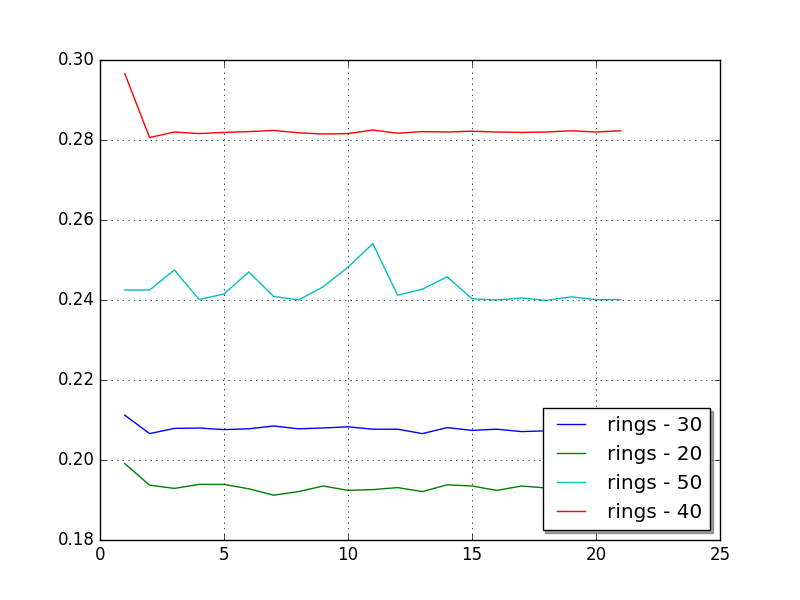
\includegraphics[width=2.5in]{_img/report_4/img_results_ps3_rings.png}
\caption{Results of RMS vs iterations in PS3 camera and rings pattern}
\end{figure}

\begin{figure}[H]
\centering
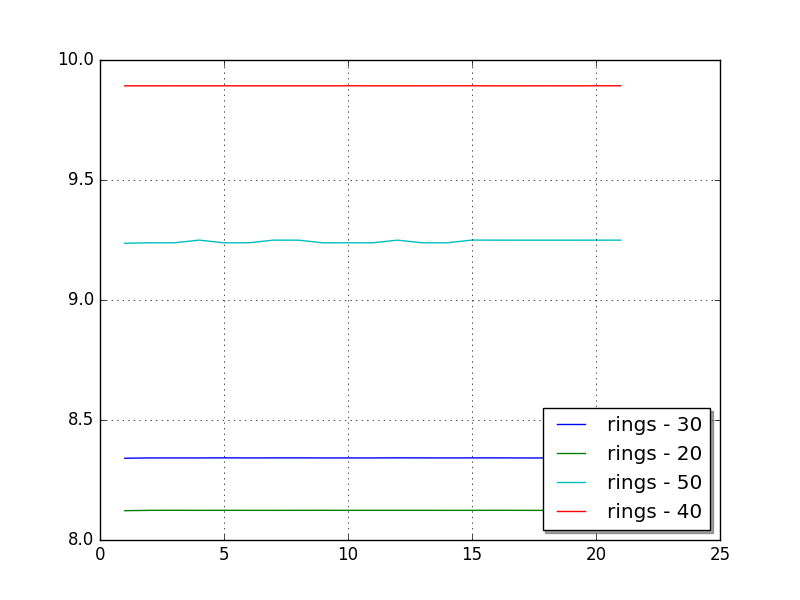
\includegraphics[width=2.5in]{_img/report_4/img_results_ps3_colinearity_rings.png}
\caption{Results of colinearity error vs iterations in PS3 camera and rings pattern}
\end{figure}


\section{Conclusions}

\begin{itemize}

    \item By the results we see that the refinement helps a little in the concentric pattern case. We see a small drop in the RMS error in this pattern with the PS3 camera. It seems that this approach doesn't help very much in the case of the other patterns, being the chessboard the case in which in fact increases the error. This could be because of the initial calibration, as for some tests we did with poorly calibrated cases we saw that the iterative process made the intrinsic parameters ( mainly the camera center ) move around a region in a random way.

    \item We can conclude that the refinement process helps, but very little, as the plots suggest. This could be caused by the choice of the refined points, as we are only integrating the refined points into the new refined batch. One way to fix this could be to use more information of the pattern in te fronto parallel view, to generate an extra set of points ( expected grid pattern ) which could be averaged with the refined points and the previous pattern points.

    \item After testing the refinement, we also noticed that the distribution of the frames taken for the calibration plays a big role in a good calibration process. We noticed this by plotting the error and checking which frames caused more reprojection error in the batch, as you can see in the following picture.

    \begin{figure}[H]
    \centering
    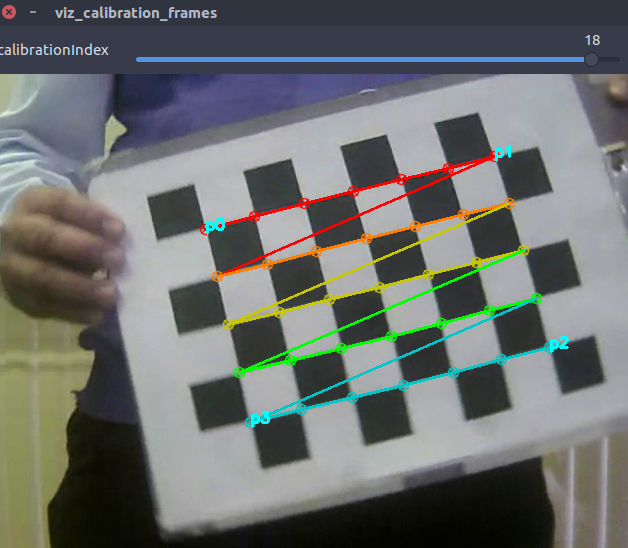
\includegraphics[width=1.5in]{_img/report_4/img_issue_frames_distribution_1.png}
    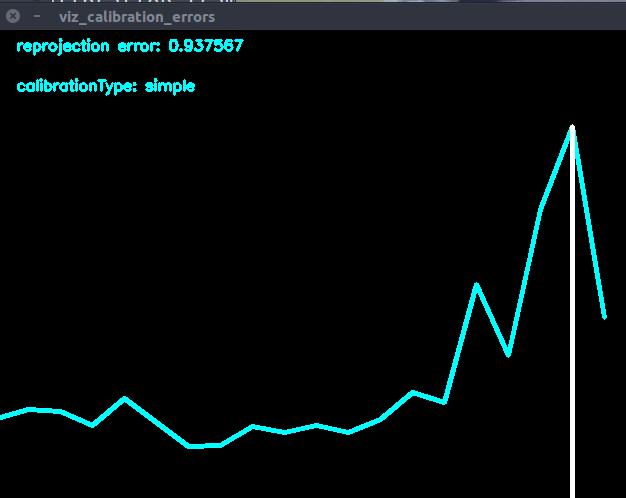
\includegraphics[width=1.5in]{_img/report_4/img_issue_frames_distribution_1_plot.png}
    \caption{A frame not uniform to the calibration batch generates bigger reprojection errors}
    \end{figure}    

    As shown in the previous figure, this was a frame that didn't have much correlation with the other frames in the batch, as it was closer to the camera than the other. This suggests that a good calibration should be one that takes frames uniformly not only in the \textbf{x, y} axes, but in the \textbf{z} axis as well ( the cloud of points representing the frames should be uniformly distributed around the \textbf{xyz} region ).

    \item We also checked that a multithreaded implementation allowed easy extraction of the information and a more responsive way to implement calibration. Our first implementation lacked this featured, and it was not possible to analyze other aspects of the previous results while we were waiting for the results, nor we could see intermediate results as the iterations passed. The calibration process can be easily parallelized - extracted from the application thread, as it only needs to be working on an initial set of features and then not touching other applications' data.

\end{itemize}

\IEEEtriggeratref{8}

% references section
\begin{thebibliography}{1}

\bibitem{OpenCV}
  Bradski, G. \\
  \textit{OpenCV library.} - 2000
\\
\bibitem{Prakash2012}
  Charan Prakash, Lina Karam\\
  \textit{Camera calibration using adaptive segmentation and ellipse fitting for localizing control points.} - 2012
\\
\bibitem{Ankur2009}
  Ankur Datta, Jun-Sik Kim, Takeo Kanade\\
  \textit{Accurate camera calibration using iterative refinement of control points.} - 2009
\\
\bibitem{CameraCalibration1}
  Zhengyou Zhang \\
  \textit{A Flexible New Technique for Camera Calibration.} - 2000
\\
\bibitem{IntegralImageThresholding}
  Derek Bradley, Gerhard Roth \\
  \textit{Adaptive Thresholding Using the Integral Image.} - 2011

\end{thebibliography}


\end{document}
